% SENTINEL — workshop paper (IEEE conference format).
% Every number in this paper is a macro from numbers.tex, which is GENERATED
% from the result files by ../research/make_numbers.py. Do not type numbers by
% hand: regenerate instead, so that every figure traces to a result file.
\documentclass[conference]{IEEEtran}
\IEEEoverridecommandlockouts
\usepackage{cite}
\usepackage{amsmath,amssymb}
\usepackage{graphicx}
\usepackage{booktabs}
\usepackage{multirow}
\usepackage{url}
\usepackage{xcolor}
\usepackage{tikz}
\usetikzlibrary{arrows.meta,positioning,fit,calc,shapes.geometric}
\usepackage{pgfplots}
\pgfplotsset{compat=1.17}
\usepackage[hidelinks]{hyperref}

% GENERATED by research/make_numbers.py from research/results — do not edit.
\newcommand{\NabuseS}{0.73}
\newcommand{\NattackWindows}{650{,}631}
\newcommand{\NblindShare}{27.8\%}
\newcommand{\NdeplAUCout}{0.983}
\newcommand{\NdeplEnnioFPR}{0.66\%}
\newcommand{\NdeplFPRout}{4.42\%}
\newcommand{\NdeplMissedShare}{27.6\%}
\newcommand{\NdeplPhilipsFPR}{5.46\%}
\newcommand{\NdeplTPR}{72.4\%}
\newcommand{\NdeplTcp}{0.71\%}
\newcommand{\NdeplThr}{0.00400}
\newcommand{\NdeplUdp}{0.36\%}
\newcommand{\NdetectPPS}{6{,}400}
\newcommand{\NenfBlock}{16.0}
\newcommand{\NenfBlockP}{32.1}
\newcommand{\NenfUnblock}{96.1}
\newcommand{\NlatBus}{0.120}
\newcommand{\NlatDetectPkt}{0.156}
\newcommand{\NlatExtract}{0.073}
\newcommand{\NlatInfer}{0.083}
\newcommand{\NlatPolicy}{0.486}
\newcommand{\NllmAsbBlock}{87.1\% [71.1, 94.9]}
\newcommand{\NllmAsbJson}{100.0\%}
\newcommand{\NllmAsbN}{31}
\newcommand{\NllmAsbTac}{0.0\% [0.0, 11.0]}
\newcommand{\NllmAsbTech}{0.0\% [0.0, 11.0]}
\newcommand{\NllmAsbTechDisc}{0.0\% [0.0, 39.0]}
\newcommand{\NllmAsbTechDos}{0.0\% [0.0, 13.3]}
\newcommand{\NllmAsbTechFlag}{0.0\% [0.0, 12.5]}
\newcommand{\NllmAsbTopTech}{T1071 (26), T1190 (3), T1071.001 (1)}
\newcommand{\NllmCold}{44.9}
\newcommand{\NllmEviBlock}{79.5\% [64.5, 89.2]}
\newcommand{\NllmEviJson}{100.0\%}
\newcommand{\NllmEviN}{39}
\newcommand{\NllmEviTac}{2.6\% [0.5, 13.2]}
\newcommand{\NllmEviTech}{0.0\% [0.0, 9.0]}
\newcommand{\NllmEviTechDisc}{0.0\% [0.0, 35.4]}
\newcommand{\NllmEviTechDos}{0.0\% [0.0, 10.7]}
\newcommand{\NllmEviTechFlag}{0.0\% [0.0, 11.0]}
\newcommand{\NllmEviTopTech}{T1071.001 (18), T1071 (16)}
\newcommand{\NllmFlagN}{31}
\newcommand{\NllmLatMed}{9.8}
\newcommand{\NllmLatP}{11.9}
\newcommand{\NllmN}{70}
\newcommand{\NlstmFPRin}{\textbf{??}}
\newcommand{\NlstmFPRout}{\textbf{??}}
\newcommand{\NotxFullMax}{152}
\newcommand{\NotxFullMed}{21.5}
\newcommand{\NotxFullMin}{7.2}
\newcommand{\NotxFullN}{5}
\newcommand{\NotxGenMed}{0.36}
\newcommand{\NotxGenN}{10}
\newcommand{\NotxSpeedup}{60}
\newcommand{\NparNewHw}{100.00\%}
\newcommand{\NparNewMag}{100.00\%}
\newcommand{\NparNewMih}{99.99\%}
\newcommand{\NparNewPcc}{100.00\%}
\newcommand{\NparNewPccN}{47{,}479}
\newcommand{\NparNewRad}{100.00\%}
\newcommand{\NparOldHw}{100.00\%}
\newcommand{\NparOldMag}{100.00\%}
\newcommand{\NparOldMih}{98.70\%}
\newcommand{\NparOldPcc}{100.00\%}
\newcommand{\NparOldPccN}{2}
\newcommand{\NparOldRad}{45.47\%}
\newcommand{\NparPackets}{55{,}318}
\newcommand{\NprovRows}{322{,}064}
\newcommand{\TperAttackRows}{Mirai & scan & 99.9 & \textbf{??} & \textbf{??} & \textbf{??} \\
Mirai & ack & 100.0 & \textbf{??} & \textbf{??} & \textbf{??} \\
Mirai & syn & 100.0 & \textbf{??} & \textbf{??} & \textbf{??} \\
Mirai & udp & 100.0 & \textbf{??} & \textbf{??} & \textbf{??} \\
Mirai & udpplain & 100.0 & \textbf{??} & \textbf{??} & \textbf{??} \\
BASHLITE & scan & 100.0 & \textbf{??} & \textbf{??} & \textbf{??} \\
BASHLITE & junk & 100.0 & \textbf{??} & \textbf{??} & \textbf{??} \\
BASHLITE & combo & 100.0 & \textbf{??} & \textbf{??} & \textbf{??} \\
BASHLITE & tcp & 0.7 & \textbf{??} & \textbf{??} & \textbf{??} \\
BASHLITE & udp & 0.4 & \textbf{??} & \textbf{??} & \textbf{??} \\}


\begin{document}

\title{SENTINEL: A Local-LLM Detection-to-Response\\Pipeline for Home IoT, and the\\Evaluation Pitfalls It Exposed}

% AUTHOR BLOCK: placeholders are deliberate — confirm full name, affiliation
% and contact e-mail before submission. Nothing here was inferred.
\author{
\IEEEauthorblockN{Vinay Sharma\textsuperscript{1}, Shyamjee Rai\textsuperscript{2}, Naman Rai\textsuperscript{3}, Neha Nilawar\textsuperscript{4}, Nikhilesh Mankar\textsuperscript{5}}
\IEEEauthorblockA{\textsuperscript{1,2,3,4}Dept. of CSE, School of Engineering and Technology,\\
Pimpri Chinchwad University (PCU), Pune, Maharashtra, India\\
\textsuperscript{5}[Affiliation — confirm]\\
\{email1, email2, email3, email4, email5\}}
}

\maketitle

% TODO: abstract (written after results)

\section{Introduction}
\label{sec:intro}

Consumer Internet-of-Things devices are numerous, rarely patched, and
frequently exposed on home networks with default credentials. The Mirai botnet
showed the consequence at scale: a large population of cameras, routers and
recorders was conscripted into denial-of-service attacks largely by guessing
factory passwords~\cite{antonakakis2017mirai}. A household has no security
operations team to watch its traffic. Whatever defends it has to run
unattended, on modest hardware, and without shipping private traffic to a
third party.

This paper describes \textsc{Sentinel}, an open-source appliance that attempts
exactly that, and reports what a careful evaluation of it revealed.
\textsc{Sentinel} captures traffic on the home segment, scores it with an
autoencoder over Kitsune's streaming features~\cite{mirsky2018kitsune}, asks a
locally hosted large language model (LLM) to label anomalous events with MITRE
ATT\&CK tactics and techniques~\cite{mitreattack}, and turns the label into an
nftables~\cite{nftables} block through a deterministic, auditable response
policy. Honeypots~\cite{cowrie,opencanary} feed attacker addresses into the
same enforcement path. The language model runs on the appliance itself, so no
packet payload or traffic content leaves the home.

Building such a pipeline is now easy; knowing whether it works is not. Anomaly
detectors for IoT traffic are routinely reported at near-perfect accuracy on
public benchmarks, yet aggregate scores on lab datasets say little about how a
system behaves when deployed~\cite{sommer2010closedworld,arp2022dosdonts}. We
therefore treated evaluation as the main object of study, and it overturned
several things we believed about our own system:

\begin{itemize}
\item \emph{A per-class blind spot hidden by the aggregate.} On
  N-BaIoT~\cite{meidan2018nbaiot}, the deployed detector catches the Mirai
  attacks almost perfectly, yet misses nearly all BASHLITE TCP and UDP floods,
  which make up \NblindShare{} of attack windows. An aggregate
  detection rate conceals this entirely.
\item \emph{False positives grow on unseen devices.} Holding out entire devices
  from training, as a new gadget joining a home network would be, raises the
  false-positive rate from \NlstmFPRin{} to \NlstmFPRout{} for our
  reproducible model.
\item \emph{The live feature extractor did not match the training features.}
  \textsc{Sentinel}'s own re-implementation of the Kitsune extractor computed
  40 of the 115 features differently from the data the model was trained on,
  so offline accuracy did not describe the running system. We traced the
  discrepancy, fixed it by adopting the reference implementation, and verified
  parity against invariants measured on the training data itself.
\item \emph{The LLM's labels were almost never right.} In a pre-registered
  test, the local model named a correct ATT\&CK technique for
  \NllmAsbTech{} of attack windows, labelling \NllmCtwoShare{} of all
  events as Command and Control; describing the traffic to it did not help.
  Because the response policy acts on the model's severity, which it set high
  for most events, the pipeline would still have blocked \NllmAsbBlock{} of
  attacks---for reasons unrelated to the label.
\end{itemize}

\noindent Our contributions are:
\begin{enumerate}
\item The design and open-source implementation of an end-to-end,
  on-premise detection-to-response pipeline for home IoT networks that keeps
  inference, including the LLM, on the appliance (\S\ref{sec:design}).
\item A leakage-aware evaluation protocol for N-BaIoT with a
  \emph{held-out-device} split, applied to the deployed model, a reproducible
  retraining over five seeds, and two baselines (\S\ref{sec:method},
  \S\ref{sec:res-detect}).
\item A pre-registered evaluation of LLM ATT\&CK labelling on the events the
  pipeline actually produces, with and without a traffic summary, showing that
  a small local model does not yet perform this task (\S\ref{sec:res-llm}).
\item A per-stage latency breakdown on a four-core aarch64 host, locating the
  bottleneck of the detection-to-response path (\S\ref{sec:res-latency}).
\item Practical lessons for building and evaluating such systems: recovering
  the provenance of an undocumented model from its scaler, and checking that
  live features match training features (\S\ref{sec:discussion}).
\end{enumerate}

All code, the evaluation harness, the pre-registration and the result files
are released with the system.\footnote{Repository URL withheld for review.}

\section{Background and Related Work}
\label{sec:related}

\paragraph{Anomaly detection for IoT traffic}
Kitsune introduced a family of damped, incremental statistics computed per
packet over several time scales and several stream aggregations (host,
MAC--IP pair, channel, socket), together with an ensemble of small
autoencoders that learns benign behaviour online~\cite{mirsky2018kitsune}. It
was designed for resource-constrained network devices and evaluated on a
Raspberry~Pi. N-BaIoT applied the same 115 features to traffic captured from
nine commercial IoT devices before and after infection by the Mirai and
BASHLITE botnets, training one deep autoencoder per device and reporting that
all attacks were detected~\cite{meidan2018nbaiot}. Newer benchmarks such as
CICIoT2023 cover more devices and attack types~\cite{neto2023ciciot}.
\textsc{Sentinel} reuses the Kitsune feature definition and the N-BaIoT data,
but trains a single sequence autoencoder shared across devices, which is the
realistic choice for an appliance that cannot collect labelled benign traffic
for every new gadget in advance.

\paragraph{How such detectors are evaluated}
Sommer and Paxson argued that anomaly detection for networks is harder than
the machine-learning framing suggests: the cost of false positives is high,
the semantic gap between an anomaly and an attack is wide, and evaluation data
rarely resembles deployment~\cite{sommer2010closedworld}. Arp~et~al.\
catalogue recurring pitfalls in security machine learning, among them data
snooping, spurious correlations, inappropriate baselines and misleading
metrics under class imbalance~\cite{arp2022dosdonts}, and dataset audits have
found labelling and construction errors in widely used intrusion
datasets~\cite{engelen2021cicids}. Our evaluation is an application of that
advice to a complete system rather than to a single model; several of the
problems we report are instances of the pitfalls they describe.

\paragraph{LLMs for security operations}
Large language models are increasingly applied to security tasks, including
threat-intelligence extraction and mapping to ATT\&CK; a recent systematic
review surveys this literature~\cite{xu2025llmsec}, and surveys of ATT\&CK's
use in research describe the mapping problem in
detail~\cite{roy2023sok,alsada2023attack}. Agentic designs that chain
detection, classification and response have also appeared; AgenticCyber, for
instance, orchestrates cloud-hosted multimodal models over enterprise
telemetry~\cite{roy2025agenticcyber}. \textsc{Sentinel} differs in placing a
small quantised model on the appliance itself, which removes the need to send
traffic to a cloud service but constrains model size and speed. Most prior
evaluations of LLM ATT\&CK mapping use written threat reports as input; we
evaluate the model on the structured anomaly events a detector actually
produces.

\paragraph{Deception and automated blocking}
Honeypots are a long-standing source of attacker intelligence for IoT.
HoneyIoT adapts a high-interaction IoT honeypot's responses with
reinforcement learning to prolong attacker engagement~\cite{guan2023honeyiot}.
Heiding~et~al.\ used honeypot observations to evaluate login blocking for IoT
devices~\cite{heiding2020honeypot}, so feeding deception data into blocking is
not new. \textsc{Sentinel}'s contribution here is integration rather than
invention: honeypot sessions and detector alerts share one enforcement path
with one safety guard.

\paragraph{Kernel-level enforcement}
eBPF and XDP allow packets to be filtered in the kernel's fast path.
iKern embeds intrusion detection and prevention in eBPF~\cite{hadi2024ikern},
Zhang~et~al.\ run a neural network inside the kernel for real-time
prevention~\cite{zhang2024ebpf}, and eBPF-based DDoS mitigation has been
demonstrated on a Raspberry~Pi~4~\cite{tolay2025ebpf}. \textsc{Sentinel}
keeps all learning in user space and uses nftables for enforcement; it
contains an XDP drop path, but that path was not enabled in the configuration
evaluated here.

\paragraph{Home IoT context}
IoT Inspector collected labelled traffic from smart-home devices at scale and
found device behaviour to be comparatively regular~\cite{huang2020iotinspector},
which is the premise of anomaly detection on the home segment. Manufacturer
Usage Descriptions let vendors declare the traffic a device
needs~\cite{lear2019mud}; they are complementary to anomaly detection, but
require manufacturer participation that most consumer devices lack.

\section{System Design}
\label{sec:design}

\textsc{Sentinel} is a set of cooperating services on one host, connected by
a Redis publish/subscribe bus (Fig.~\ref{fig:arch}). We describe the system as
built and evaluated, which differs in places from its original design; where
it does, we say so.

\begin{figure}[t]
\centering
\resizebox{\columnwidth}{!}{% SENTINEL architecture — the detection-to-response path as built.
% Solid boxes run on the appliance; dashed boxes are external services.
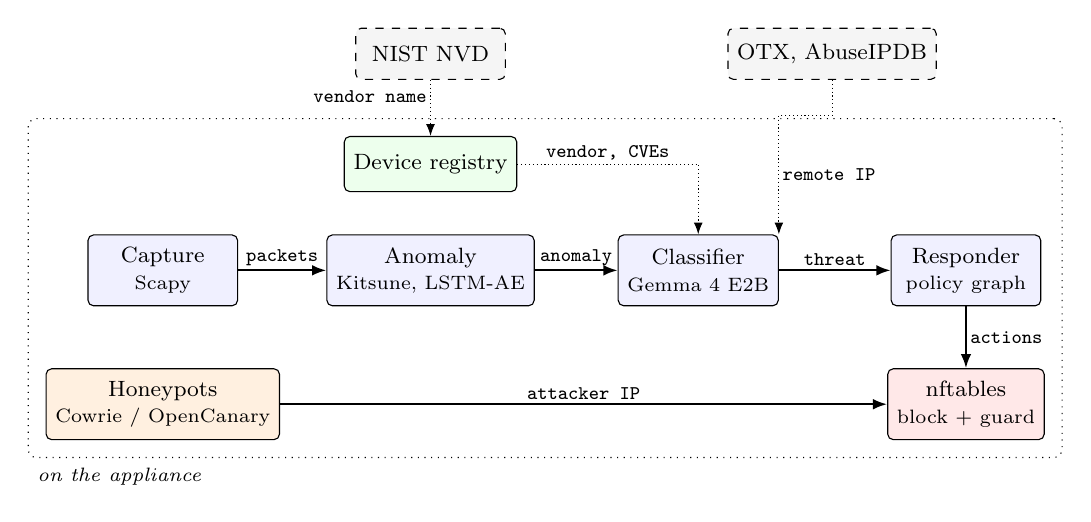
\begin{tikzpicture}[
  font=\footnotesize,
  stage/.style={draw, rounded corners=2pt, align=center, minimum height=9mm,
                minimum width=19mm, fill=blue!6},
  ext/.style={draw, dashed, rounded corners=2pt, align=center, minimum height=6.5mm,
              minimum width=19mm, fill=gray!8},
  bus/.style={-{Latex[length=1.8mm]}, thick},
  side/.style={-{Latex[length=1.5mm]}, densely dotted},
  lbl/.style={font=\scriptsize\ttfamily, inner sep=1.2pt}
]
% main path (y = 0), 34 mm pitch leaves room for the channel labels
\node[stage] (cap) at (0,0)    {Capture\\{\scriptsize Scapy}};
\node[stage] (ano) at (3.4,0)  {Anomaly\\{\scriptsize Kitsune, LSTM-AE}};
\node[stage] (cls) at (6.8,0)  {Classifier\\{\scriptsize Gemma 4 E2B}};
\node[stage] (rsp) at (10.2,0)  {Responder\\{\scriptsize policy graph}};
\draw[bus] (cap) -- node[lbl, above] {packets} (ano);
\draw[bus] (ano) -- node[lbl, above] {anomaly} (cls);
\draw[bus] (cls) -- node[lbl, above] {threat}  (rsp);

% enforcement row (y = -1.7)
\node[stage, fill=orange!12] (hp) at (0,-1.7)   {Honeypots\\{\scriptsize Cowrie / OpenCanary}};
\node[stage, fill=red!9]     (fw) at (10.2,-1.7) {nftables\\{\scriptsize block + guard}};
\draw[bus] (rsp) -- node[lbl, right] {actions} (fw);
\draw[bus] (hp) -- node[lbl, above] {attacker IP} (fw);

% local registry (on the appliance), above the main path
\node[stage, fill=green!7, minimum height=7mm] (reg) at (3.4,1.35) {Device registry};
\draw[side] (reg.east) -| node[lbl, above, pos=0.25] {vendor, CVEs} (cls.north);

% the appliance boundary
\node[draw, dotted, rounded corners=3pt, inner xsep=2.2mm, inner ysep=2.2mm,
      fit=(cap)(rsp)(hp)(fw)(reg)] (box) {};
\node[font=\scriptsize\itshape, anchor=north west] at (box.south west) {on the appliance};

% external services, above the boundary
\node[ext] (nvd)   at (3.4,2.75) {NIST NVD};
\node[ext] (intel) at (8.5,2.75) {OTX, AbuseIPDB};
\draw[side] (nvd) -- node[lbl, left, pos=0.3] {vendor name} (reg);
\draw[side] (intel.south) |- ++(0,-0.45) -| node[lbl, right, pos=0.75] {remote IP} (cls.north east);
\end{tikzpicture}
}
\caption{The detection-to-response path. Solid arrows are bus channels;
dashed boxes are the only components that contact external services.}
\label{fig:arch}
\end{figure}

\subsection{Capture and device context}
A capture service reads packets from the monitored interface with Scapy's
asynchronous sniffer and publishes a compact per-packet record (addresses,
ports, length, timestamp) on the bus. A discovery service builds a device
registry passively from the mDNS, SSDP, DHCP and ARP traffic it observes, maps
MAC prefixes to vendors, and queries NIST's National Vulnerability Database for
known CVEs by vendor. Active Nmap scanning exists but is triggered only on
demand from the dashboard.

\subsection{Anomaly detection}
For every packet the anomaly service computes the 115 Kitsune
features~\cite{mirsky2018kitsune}: damped statistics at five time scales
($\lambda \in \{5, 3, 1, 0.1, 0.01\}$) over five stream aggregations (source
MAC--IP pair, source IP, channel, channel jitter, and socket), including
two-dimensional statistics that relate each channel or socket to its reverse
direction. It keeps a sliding window of the last ten feature vectors per
device and scores each full window with a sequence autoencoder: a two-layer
LSTM~\cite{hochreiter1997lstm} encoder compresses the $10\times115$ window into
a 64-dimensional state, which is repeated across ten steps and decoded by a
second two-layer LSTM and a linear layer (153,651 parameters in total). The
anomaly score is the mean squared reconstruction error over the whole window,
computed with ONNX Runtime~\cite{onnxruntime} on min--max-scaled features, and
an event is raised when it exceeds a single threshold shared by all devices.

\subsection{LLM classification}
The classifier service enriches each anomaly event with the device's vendor
and known CVEs from the registry and with the reputation of the remote address
from AlienVault OTX~\cite{otx} and AbuseIPDB~\cite{abuseipdb}. It then asks
Gemma~4~E2B~\cite{gemma4}, served locally by Ollama~\cite{ollama} and quantised
to 4 bits, for a JSON object with an ATT\&CK tactic and technique identifier,
a confidence, a severity from 1 to 10, a one-sentence summary and a
recommended action. The model runs with Ollama's default sampling
(temperature~1.0), so its output for a given event is not deterministic.
Events whose response does not parse are dropped.

\subsection{Response and enforcement}
The response service is a two-node LangGraph~\cite{langgraph} state machine,
not a second language model: a policy node maps the LLM's severity to actions
through a declarative policy file, and a gate node holds the action for human
confirmation when the policy requires it. In the evaluated configuration,
severities 6--10 cause the event's indicator address---the destination of the
anomalous flow---to be blocked without confirmation, and lower severities are
logged. The policy also names a device-quarantine action for severities 9--10;
the responder currently enforces it as the same address block, and a
MAC-level quarantine module exists but is not invoked by the responder. Keeping the enforcement decision deterministic and
inspectable, rather than generated, is deliberate: the model proposes a
severity, and a policy the owner can read decides what happens.

Blocks are applied as nftables rules in a dedicated table, each tracked by its
rule handle so that it can be removed individually. A guard refuses to block
the appliance's own addresses, the default gateway, loopback, broadcast and
unspecified addresses, and address ranges, so that a misclassification cannot
cut the home off its own router. An XDP fast path is implemented but was not
enabled for this evaluation.

\subsection{Deception}
Cowrie~\cite{cowrie} (SSH and Telnet) and OpenCanary~\cite{opencanary} run in
containers. A honeypot service follows Cowrie's JSON log, records credentials
and commands from each session as a threat event, and sends the attacker's
address to the same guarded enforcement path.

\subsection{What leaves the appliance}
No packet payload, capture or feature vector is sent off the device, and the
LLM runs locally. Three lookups do leave it: the remote address of each
anomalous flow goes to OTX and AbuseIPDB, and device vendor names go to the
NVD. All three are optional, and a privacy-sensitive deployment can disable
them at some cost to context.

\subsection{Threat model}
In scope are network-observable attacks involving devices on the monitored
segment: compromised devices scanning or flooding (as in N-BaIoT), and inbound
credential attacks against exposed services (as seen by the honeypots). We
assume the attacker does not control the appliance and cannot tamper with its
view of the traffic. Out of scope are physical access, inspection of encrypted
payloads, supply-chain compromise, attacks on \textsc{Sentinel} itself, and
adaptive attackers who shape traffic to evade the detector.

\section{Evaluation Methodology}
\label{sec:method}

\subsection{Dataset and the deployed model's provenance}
We evaluate detection on N-BaIoT~\cite{meidan2018nbaiot}: benign traffic from
nine commercial devices (doorbells, a thermostat, a baby monitor, security
cameras and a webcam) and traffic from the same devices after infection by
Mirai and BASHLITE, each executing five attacks. Features are the 115 Kitsune
statistics described in \S\ref{sec:design}. The attack classes are defined by
the dataset's authors; for example, BASHLITE \emph{COMBO} is ``sending spam
data and opening a connection to a specified IP address and port'' and Mirai
\emph{UDPplain} is ``UDP flooding with fewer options, optimized for higher
PPS''~\cite{meidan2018nbaiot}.

The model shipped with \textsc{Sentinel} had been trained in a notebook that
was not kept, so its training data was undocumented. We recovered it from the
saved min--max scaler: its 115 per-feature minima and maxima match the benign
traffic of exactly six of the nine devices with zero deviation, and the number
of rows it was fitted on (\NprovRows{}) equals their combined benign row count.
We call these six devices \emph{in-distribution} and the remaining three
(\emph{Ennio} doorbell, \emph{Philips} baby monitor, \emph{SimpleHome} XCS7-1003
camera) \emph{held-out}. No model evaluated here saw any traffic from the
held-out devices, which therefore measure how the detector behaves on a device
it has never observed---the ordinary case for a home appliance.

\subsection{Splits and leakage}
Adjacent rows of Kitsune features share damped statistics, so a random
train/test split places near-duplicate rows on both sides of the boundary.
Following Meidan~et~al., we split each in-distribution device's benign
traffic \emph{chronologically} and keep the final third for
testing~\cite{meidan2018nbaiot}. We train on the first 90\% of the remainder
and use the last 10\% for early stopping and threshold selection. Scalers are
fitted on the training portion only. Attack traffic is never used for training
or threshold selection. Windows are ten consecutive rows from a single capture
file, never spanning a file or device boundary; test windows do not overlap.

The deployed model does not satisfy these conditions---its scaler saw all
benign rows of the in-distribution devices---so we report its in-distribution
false-positive rate only as optimistic and rely on its held-out-device and
attack results, which are clean.

\subsection{Models compared}
\begin{itemize}
\item \emph{Deployed}: the shipped ONNX model with its shipped threshold.
\item \emph{LSTM-AE}: the same architecture retrained under the protocol above
  with five seeds. Its parameter count reproduces the deployed model's exactly.
\item \emph{Dense AE}: the per-row deep autoencoder architecture of N-BaIoT's
  authors~\cite{meidan2018nbaiot} (hidden widths 86--57--37--28, mirrored),
  scoring a window by its rows' mean error. It sees the same windows as the
  LSTM-AE but models no temporal order.
\item \emph{Isolation Forest}~\cite{liu2008iforest} on the flattened window,
  as a non-neural baseline.
\end{itemize}
Every retrained model uses the same threshold rule: the 99th percentile of its
own validation-benign scores, a nominal 1\% false-positive budget fixed without
reference to attack traffic.

\subsection{LLM classification (pre-registered)}
To avoid grading our own test cases after seeing the model's answers, we
committed the experimental design to the project repository before running the
model on any sample. The ground truth maps each N-BaIoT attack class, by its
authors' definition, to a set of acceptable ATT\&CK techniques: scans to
Network Service Discovery, Active Scanning or Remote System Discovery, and all
floods to Network or Endpoint Denial of Service. Equivalent techniques from the
ATT\&CK for ICS matrix are accepted, because \textsc{Sentinel}'s prompt asks
for that matrix. We drew 20 windows per attack class (200 in total) with a fixed
seed, from both device groups, and queried the model under two prompts:
\emph{as-built}, produced by \textsc{Sentinel}'s own prompt builder, and
\emph{evidence}, identical but for five plain-language traffic statistics
computed from the window (recent packet count, mean packet size, approximate
numbers of destination hosts and of sockets, and channel jitter). Fields that
could leak the label---the protocol, notably---were withheld from both, and
reputation lookups were disabled. We report technique and tactic accuracy with
Wilson 95\% intervals~\cite{wilson1927}, the rate of valid JSON, and latency.
Two further analyses were declared after the initial design but before any
output was seen: as a secondary analysis, results restricted to the windows the
detector would actually forward to the classifier; and, labelled exploratory,
the rate at which the pipeline would have blocked, i.e.\ the fraction of
attack windows assigned severity~$\geq 6$.

\subsection{Latency and host}
We time each stage of the path in process with the real components: feature
extraction per packet on real traffic (the Mirai capture distributed with
Kitsune~\cite{kitsunepy}), anomaly inference per window, a Redis bus hop, the
response policy, and the threat-intelligence lookups. LLM latency is taken from
the \NllmLatN{} classification calls that ran on this host. All timing
measurements ran on one host: a four-core
aarch64 virtual machine with 7.7\,GB of memory. This is the same instruction
set as, and a similar core count and memory size to, the Raspberry~Pi~5 that
\textsc{Sentinel} targets, but it is not that device: it does not reproduce the
Pi's clock speed, memory bandwidth or thermal throttling, so absolute timings
on the Pi will differ. Neural models were trained on a Colab T4 GPU.

\emph{Deviation from the pre-registration.} The first \NllmLocN{} of the
400 LLM calls ran on this host as planned; the run was then stopped at a
checkpoint because it monopolised the workstation, and the remaining
\NllmCloudN{} ran on a cloud GPU with the same model (verified by digest),
prompts and sampling. We recorded this, and its consequences, in the
repository before any cloud output existed: latency is reported from the
local calls only, and accuracy pools both hosts, with a per-host check.

\section{Results}
\label{sec:results}

\subsection{Detection, per attack class}
\label{sec:res-detect}

%%DETECTION%%

\begin{table}[t]
\centering
\caption{Detection rate (\%) per attack class, all devices pooled. LSTM-AE,
Dense AE and Isolation Forest are means over five seeds.}
\label{tab:per-attack}
\footnotesize
\setlength{\tabcolsep}{4pt}
\begin{tabular}{llrrrr}
\toprule
Botnet & Attack & Deployed & LSTM-AE & Dense AE & I.\,Forest \\
\midrule
\TperAttackRows
\bottomrule
\end{tabular}
\end{table}

\begin{figure}[t]
\centering
% Detection rate per attack class. Data: figures/per_attack.csv (generated).
% Palette: categorical slots 1-4 (validated for CVD; relief = legend + Table).
\begin{tikzpicture}
\begin{axis}[
  width=\columnwidth, height=46mm,
  ybar, bar width=2.1pt,
  table/col sep=comma, unbounded coords=discard,
  ymin=0, ymax=105, ytick={0,25,50,75,100},
  ylabel={detected (\%)}, ylabel style={font=\footnotesize},
  xtick=data, xticklabels from table={figures/per_attack.csv}{label},
  xticklabel style={rotate=40, anchor=east, font=\scriptsize},
  yticklabel style={font=\scriptsize},
  ymajorgrids, grid style={gray!20},
  axis line style={gray!60}, tick style={gray!60},
  enlarge x limits=0.06,
  legend style={font=\scriptsize, at={(0.5,1.03)}, anchor=south, legend columns=4, draw=none},
  legend image code/.code={\draw[#1, draw=none] (0cm,-0.08cm) rectangle (0.22cm,0.12cm);},
]
\addplot[fill={rgb,255:red,42;green,120;blue,214}]  table[x=cls, y=deployed, col sep=comma] {figures/per_attack.csv};
\addplot[fill={rgb,255:red,235;green,104;blue,52}]  table[x=cls, y=lstm,     col sep=comma] {figures/per_attack.csv};
\addplot[fill={rgb,255:red,27;green,175;blue,122}]  table[x=cls, y=dense,    col sep=comma] {figures/per_attack.csv};
\addplot[fill={rgb,255:red,237;green,161;blue,0}]   table[x=cls, y=iforest,  col sep=comma] {figures/per_attack.csv};
\legend{Deployed, LSTM-AE, Dense AE, Isol.\ Forest}
\end{axis}
\end{tikzpicture}

\caption{Detection rate per attack class (M: Mirai, B: BASHLITE). Two
BASHLITE flood classes are almost entirely missed; Table~\ref{tab:per-attack}
gives the values.}
\label{fig:per-attack}
\end{figure}

\subsection{Unseen devices}
\label{sec:res-heldout}

%%HELDOUT%%

\subsection{Live feature parity}
\label{sec:res-parity}

Offline results describe the model on N-BaIoT's features; they describe the
running system only if the live extractor computes the same features. We
checked this with invariants measured on N-BaIoT's own rows, which any faithful
extractor must satisfy, on \NparPackets{} real packets from the Mirai capture
distributed with Kitsune~\cite{kitsunepy} (Table~\ref{tab:parity}). The
extractor originally shipped with \textsc{Sentinel} fed a single stream to both
sides of every two-dimensional statistic, so its correlation features took only
\NparOldPccN{} distinct values and its radius violated the bound on most
packets. After replacing it with the reference statistics engine and pinning
the stream layout to what the data shows, every invariant holds and the
correlation features take \NparNewPccN{} distinct values within $[-1,1]$.

\begin{table}[t]
\centering
\caption{Invariants measured on N-BaIoT, checked on real traffic for the
original and the corrected live extractor (share of packets satisfying each).}
\label{tab:parity}
\footnotesize
\begin{tabular}{lrr}
\toprule
Invariant (from N-BaIoT's rows) & Original & Corrected \\
\midrule
MI$_{\text{dir}}$ = H (one IP per MAC)        & \NparOldMih & \NparNewMih \\
channel weight $\le$ host weight              & \NparOldHw  & \NparNewHw  \\
radius $\ge$ std$^2$                          & \NparOldRad & \NparNewRad \\
magnitude $\ge |$mean$|$                      & \NparOldMag & \NparNewMag \\
$|$pcc$|$ $\le 1$                             & \NparOldPcc & \NparNewPcc \\
distinct pcc values                           & \NparOldPccN & \NparNewPccN \\
\bottomrule
\end{tabular}
\end{table}

\subsection{LLM classification}
\label{sec:res-llm}

%%LLM%%

\subsection{Latency}
\label{sec:res-latency}

Table~\ref{tab:latency} gives the median time of each stage. Everything the
appliance computes itself is fast: extracting features and scoring a window
together take \NlatDetectPkt{}\,ms per packet, enough for roughly
\NdetectPPS{} packets per second on one core, and the bus hop and response
policy each cost under a millisecond. The path is dominated by two calls. The
LLM needs \NllmLatMed{}\,s per event (95th percentile \NllmLatP{}\,s), and
\NllmCold{}\,s for the first event after the model service starts. The
AlienVault OTX lookup is slower and far less predictable: a median of
\NotxFullMed{}\,s over \NotxFullN{} lookups, ranging from \NotxFullMin{}\,s to
\NotxFullMax{}\,s. It is made with a synchronous client inside the
classifier's event loop and without a timeout, so while it waits no other
event is classified. The classifier reads only the \emph{general} section of
the OTX response, yet requests every section; requesting that section alone
takes \NotxGenMed{}\,s (median of \NotxGenN{}), a \NotxSpeedup$\times$
reduction.

\begin{table}[t]
\centering
\caption{Median latency per stage on a 4-core aarch64 host.}
\label{tab:latency}
\footnotesize
\begin{tabular}{lr}
\toprule
Stage & Median \\
\midrule
Feature extraction (per packet)            & \NlatExtract\,ms \\
Anomaly inference (per window)             & \NlatInfer\,ms \\
Redis bus hop                              & \NlatBus\,ms \\
Response policy (LangGraph)                & \NlatPolicy\,ms \\
nftables block                             & \NenfBlock\,ms \\
\midrule
LLM classification (warm)                  & \NllmLatMed\,s \\
LLM first call after start                 & \NllmCold\,s \\
AbuseIPDB lookup                           & \NabuseS\,s \\
OTX lookup, all sections (as built)        & \NotxFullMed\,s \\
OTX lookup, \emph{general} section only    & \NotxGenMed\,s \\
\bottomrule
\end{tabular}
\end{table}

\section{Discussion}
\label{sec:discussion}

\subsection{Lessons}

\paragraph{Report detection per class, and per device}
%%LESSON1%%

\paragraph{Evaluate the running system, not only the model}
A model can be evaluated flawlessly on its dataset while the deployed system
feeds it something else. \textsc{Sentinel}'s extractor was written from a
description of Kitsune rather than from its code, and the error it contained
was invisible in every offline experiment, because offline experiments read
N-BaIoT's precomputed features and never touch the extractor. The check that
caught it needs no additional data: structural invariants measured on the
training set's own rows, asserted on live output. We recommend such parity
tests as a standing part of any pipeline that trains on features computed by
someone else's tool.

\paragraph{Recover what an artefact encodes}
The deployed model arrived without its training script. Its scaler recorded,
in its per-feature minima, maxima and sample count, enough to identify the
exact training devices---which in turn exposed that its in-distribution
evaluation would have been contaminated, and supplied a natural held-out-device
split. Fitted preprocessing objects are an underused source of provenance.

\paragraph{Give the model the evidence}
%%LESSON4%%

\paragraph{Latency lives in the integration}
Every component we wrote runs in well under a millisecond per event; the
detection-to-response path is slow because of an external reputation service
called in the wrong way and a language model on a CPU. Neither problem is
visible when the detector is benchmarked alone. Requesting only the needed
section of the OTX response, running it off the event loop with a timeout, and
caching per address would remove most of the reputation cost.

\subsection{Limitations and threats to validity}
\emph{Dataset.} N-BaIoT was captured in 2018 in a laboratory, with nine
devices and two botnet families; home networks today carry more devices, more
encrypted traffic and other malware. Our results characterise these attacks on
these devices. The held-out-device split measures generalisation to three
unseen devices of the same era, not to arbitrary new hardware.

\emph{Hardware.} All timings come from a four-core aarch64 virtual machine,
not a Raspberry~Pi~5. The host matches the Pi in instruction set, core count
and approximate memory, but not in clock speed, memory bandwidth or thermal
behaviour, and sustained LLM inference on the Pi will be slower. Physical
validation remains future work.

\emph{Replay, not deployment.} Detection results come from replaying captured
features, not from a live network; the parity test narrows but does not close
the gap between the two. We have not evaluated \textsc{Sentinel} against an
adaptive attacker.

\emph{LLM evaluation.} The ground truth maps attack classes to ATT\&CK
techniques by our reading of the dataset's definitions; other mappings are
defensible, which is why we accept several techniques per class and report
tactic-level accuracy as well. The model samples at temperature~1.0, so a
single run estimates, rather than fixes, its behaviour; 200 windows per prompt
give 95\% intervals no wider than about $\pm$7 percentage points.

\emph{Deception path.} The honeypot-to-firewall path was exercised
functionally, by attacking our own honeypot, but is not evaluated
quantitatively here; the appliance's own event log mixes those sessions with
synthetic events injected to test the response logic, so we do not report
counts from it.

\emph{Single threshold.} Every retrained model uses one global threshold at a
nominal 1\% false-positive budget; other operating points trade detection for
false positives differently, and the threshold-free AUC values we report
summarise that trade-off.

\subsection{Ethics}
No data about people was collected for this work. Detection experiments use
the public N-BaIoT dataset and the Mirai capture distributed with Kitsune. The
LLM experiment used reserved documentation addresses (RFC~5737), and
reputation lookups in the latency experiment were made only for such
addresses. The honeypot path was exercised only by the author, attacking the
author's own honeypot from the author's own device.

\section{Conclusion}
\label{sec:conclusion}

\textsc{Sentinel} shows that a complete detection-to-response pipeline for a
home network, including a language model, runs on a four-core, 8\,GB-class host of the kind it targets,
and that everything except the language model and one external lookup runs in
well under a millisecond per event. Its evaluation shows how much a system can
look right while being wrong in specific, consequential ways: a detector that
misses two whole attack classes behind a respectable aggregate, false alarms
concentrated on one unseen device, a live feature extractor that fed the model
inputs it was never trained on, and a local LLM whose ATT\&CK labels are almost
never correct while its severities still drive blocking.

None of these problems was visible from the headline numbers, and each was
found by a check that is cheap to run: report per class and per device, hold
out whole devices, test live features against invariants of the training data,
pre-register the LLM test, and time every stage of the path rather than the
model alone. We offer these checks, and the harness that implements them, as
the more lasting contribution. Immediate next steps are to address the
BASHLITE flood blind spot with features that capture it, to calibrate
thresholds per device class, to make the reputation lookup asynchronous and
selective, to replace free-form LLM labelling with a validated or constrained
classifier, and to repeat the timing on physical Raspberry~Pi~5 hardware.


\bibliographystyle{IEEEtran}
\bibliography{refs}

\end{document}
